Salgssystemet fungerer først og fremmest via Kasseapparat, der med en grafisk touch brugergrænseflade lader Ekspedient sælge varer til en kunde, og tage imod betaling. 

Kasseapparatet sender/henter data til/fra CentralServer, der yderligere kommunikerer med databasen. Dette gør at Kasseapparatet kan modtage et produktkatalog fra, og få gemt et salg i, databasen. 

Superbruger har igennem en grafisk brugergrænseflade adgang til Administrationssystem. Herfra kan Superbruger tilføje, slette og redigere produkter og produktkategorier i produktkataloget. Dette betyder at Administrationssystem også har en forbindelse til CentralServer.

CentralServer sørger for al kommunikation med databasen og at håndtere kommunikation til og fra alle instanser af Administrationssystem og Kasseapparat.


\begin{figure}[!h]
    \centering
    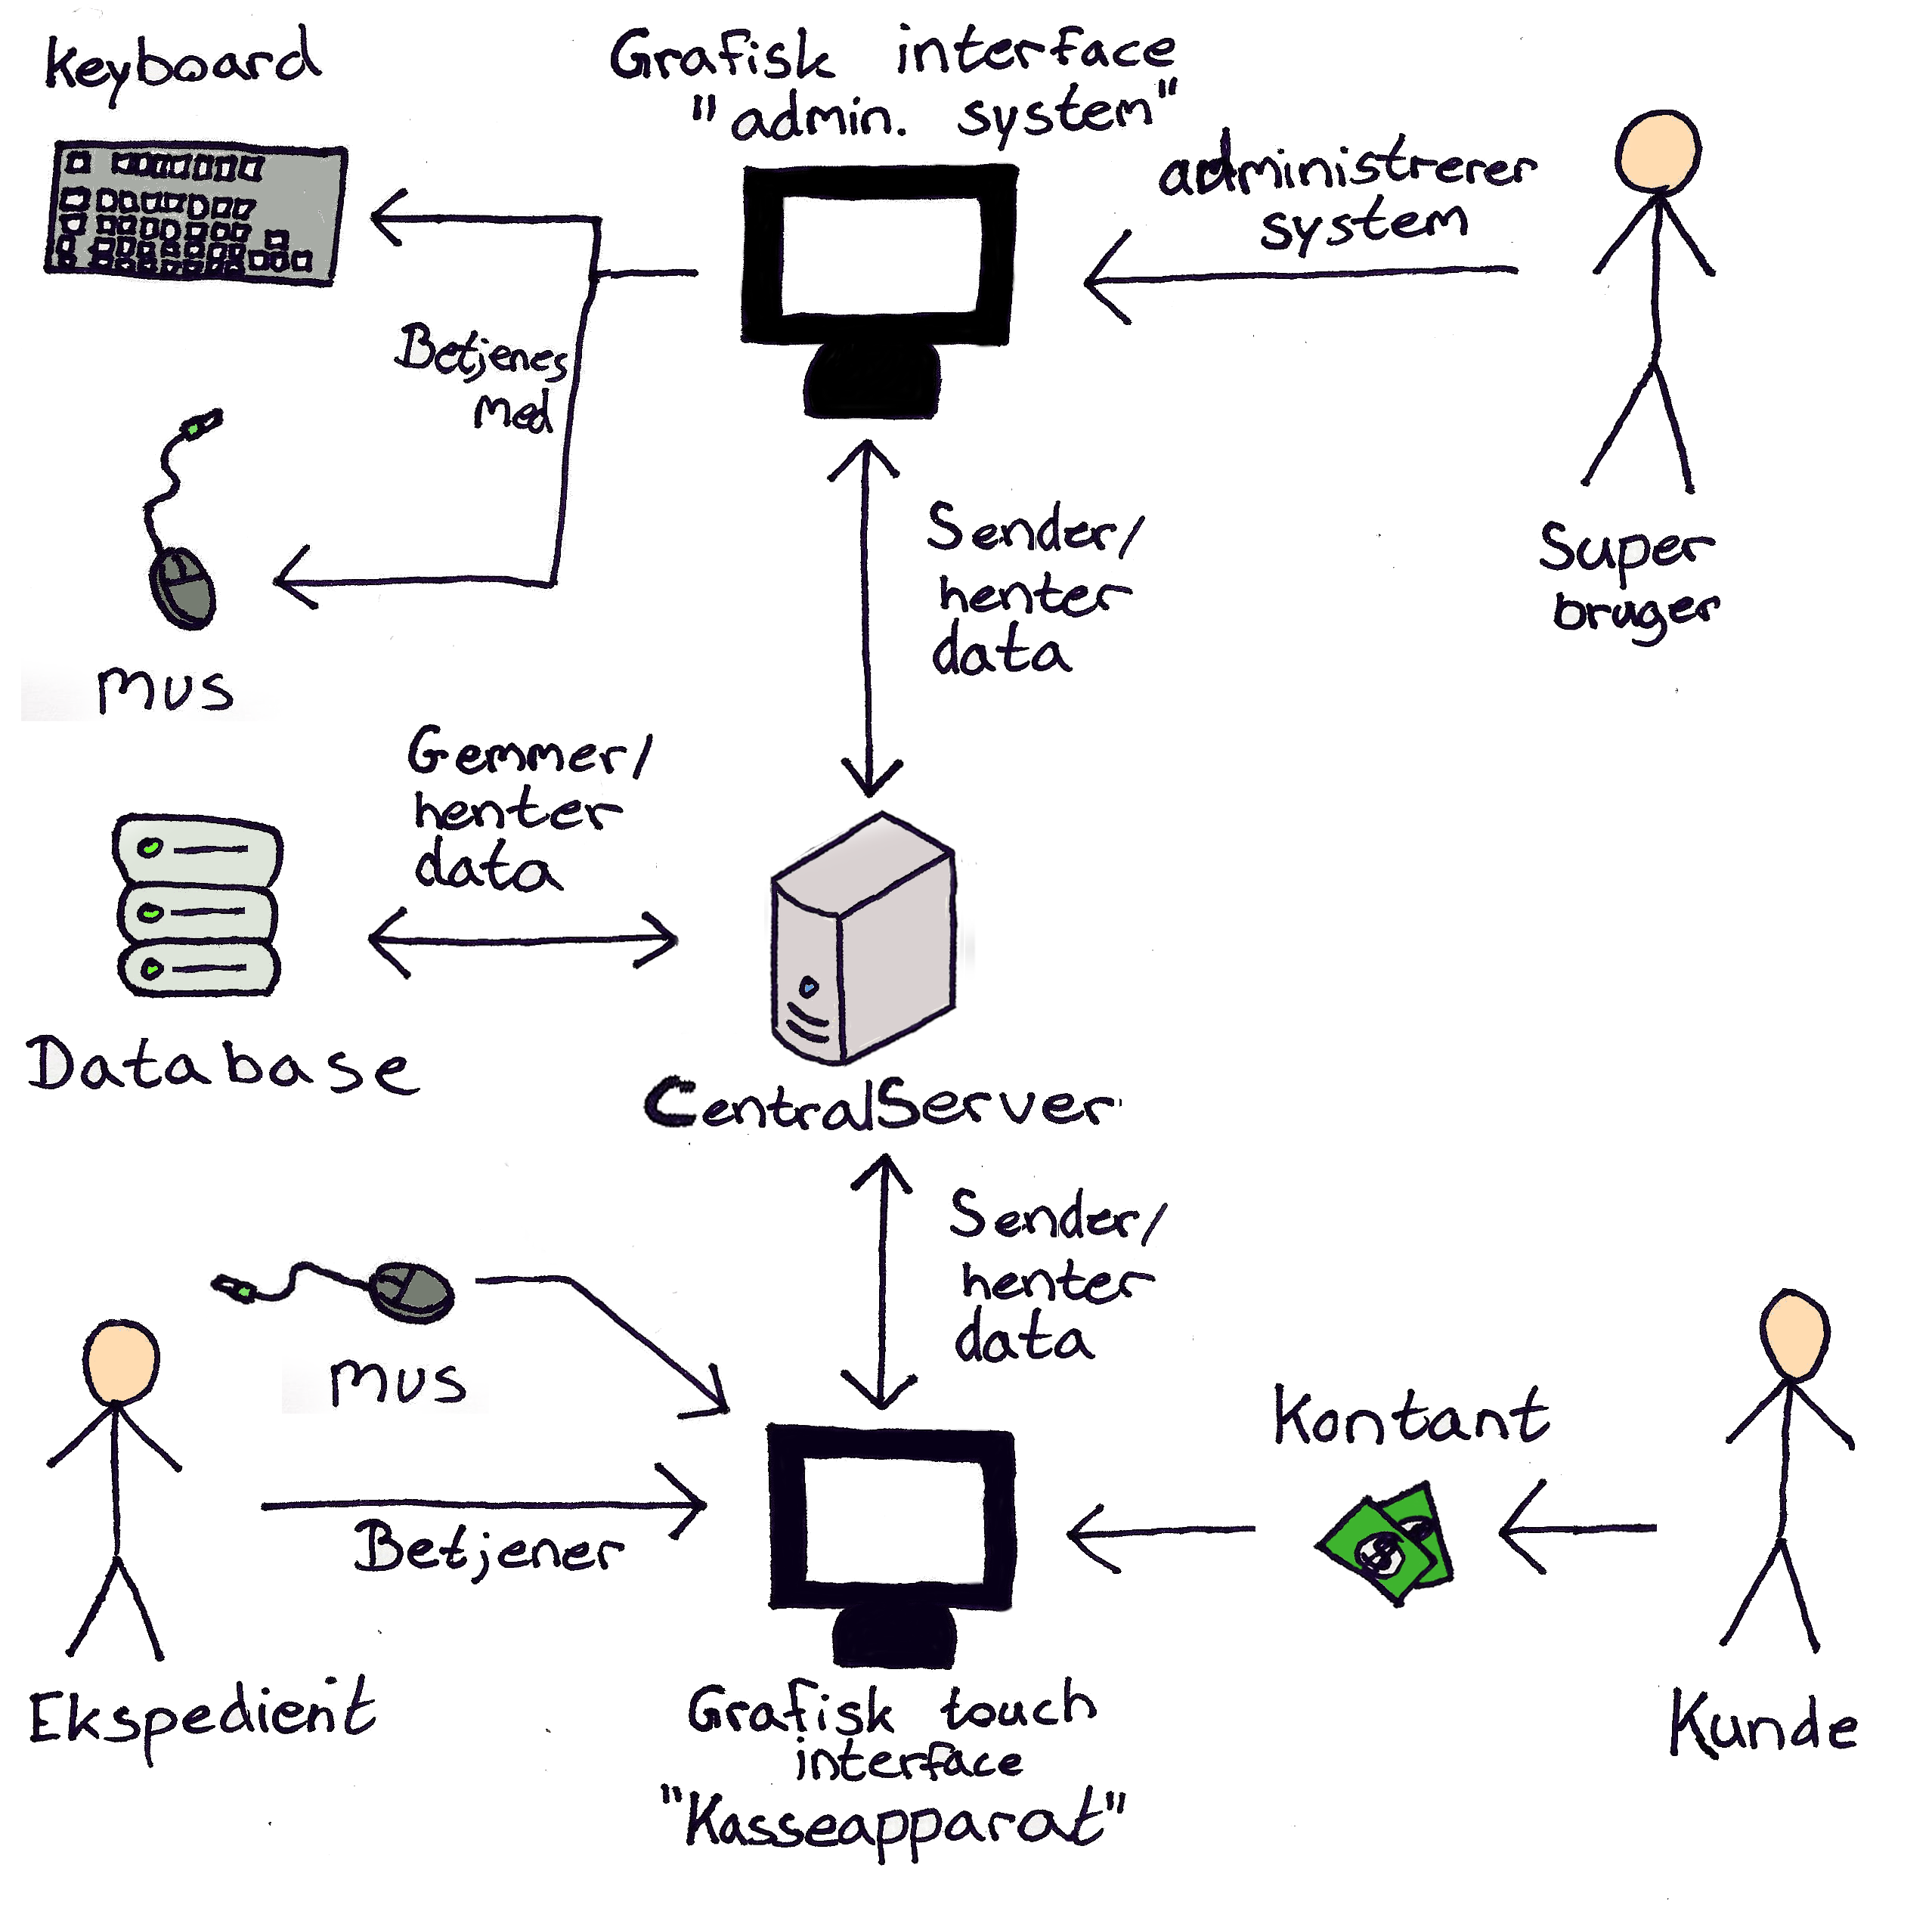
\includegraphics[width=0.8\textwidth]{Systembeskrivelse/RigtBillede3}
    \caption{Rigt billede over Salgssystemet}
    \label{fig:Rigtbill}
\end{figure}